\newcommand{\pv}[1]{
	%\ifdim#1pt<0.05pt
	%	\cellcolor{black!20}
	%\fi
	%\ifdim#1pt<0.001pt
	%	$< 0.001$
	%\else
	%	\ifdim#1pt=1.000pt
	%		\multicolumn{1}{c}{--}
	%	\else
	%		$#1$
	%	\fi
	%\fi
	#1
}
% Kronecker-structured LDA ====================================================
\begin{refsection}
	\chapter{Kronecker-structured discriminant analysis}


	Part of the work in this chapter was published in~\cite{VanDenKerchove2022}.


	\todo{Rename to LDA}
	\todo{Work Kronecker sum in}
	\todo{Add results over time vs toeplitzlda}
	\todo{Introductory part on LCMV beamforming to intro}

	\section{Introduction}

	%Brain-computer interfaces (BCIs) establish a direct communication pathway
	%between the brain and an external device~\cite{Wolpaw2002}.
	%Severely disabled patients with impaired or absent communication capabilities
	%can benefit from BCIs to restore normal functioning~\cite{Naci2012,Chaudhary2016}.
	%BCIs can be implemented in multiple ways, using non-invasive recording
	%techniques such as electroencephalography (EEG)~\cite{Abiri2019},
	%magnetoencephalography (MEG)~\cite{Mellinger2007},
	%functional Near-Infrared Spectroscopy (fNIRS)~\cite{Hong2015}, and Optically Pumped
	%Magnetometers (OPM MEG)~\cite{Paek2020}, or semi-invasive and invasive methods such as
	%electrocorticography (ECoG)~\cite{Schalk2011} or microelectrode
	%arrays~\cite{Maynard1997} which require surgery to implant a recording device.
	%While invasive BCIs yield the highest information transfer
	%rate~\cite{Willett2021}, non-invasive BCIs are preferable for short-term use
	%since they are not susceptible to the risks that come with surgery.
	%Of the non-invasive options, EEG is the most cost-effective and practical as it
	%is not limited to the same controlled settings as MEG and OPM MEG.

	%Besides the recording method, BCIs differ in the communication paradigms used
	%for communication~\cite{Abiri2019}.
	%A popular class of BCI paradigms relies on the evocation
	%of Event-Related Potentials (ERPs) in the brain in response to visual, auditory, or tactile stimulation, given their low decoding cost and generally short
	%calibration time before usage~\cite{Gao2014, Kapgate2015}.
	%The study we report on focuses on the visual P300 oddball ERP in response to a
	%rare but attended visual stimulus.
	%The decoder detects whether this ERP is present to determine which stimulus
	%the user attended.
	%The P300 paradigm has been used extensively in BCI development and is easy to
	%set up~\cite{Farwell1988, Sellers2006, Barachant2014, Philip2020}.

	There are multiple state-of-the-art P300 classification methods, like Support
	Vector Machines (SVMs)~\cite{Tayeb2014}, deep
	learning models~\cite{Vareka2020,Borra2020}, and Riemannian Geometry
	classifiers~\cite{Barachant2014}.
	While these models often return a high classification accuracy, there is a need
	for lightweight models -- lightweight models lead to fast off-line analyses and can be transferred to consumer-grade hardware.
	When moving towards plug-and-play solutions, BCI calibration sessions should be short and model training times low.
	The spatiotemporal beamformer~\cite{VanVliet2015, Wittevrongel2016} belongs to
	this class of ERP decoding models as it achieves state-of-the-art performance and is fast to train.
	Earlier work has shown that it is
	possible to apply the spatiotemporal beamformer to multiple time-locked visual
	BCI paradigms, including the P300 oddball paradigm,
	Steady-State Visually Evoked Potentials (SSVEP), code-modulated Visually Evoked Potentials (cVEP)~\cite{Wittevrongel2017a} and
	motion-onset Visually Evoked Potentials (mVEP)~\cite{Libert2021}.

	This work shows that the original spatiotemporal
	beamformer~\cite{Wittevrongel2016} can fall short in performance when BCI
	calibration data are restricted.
	We also show that the spatiotemporal beamformer does not scale well for
	higher spatial and temporal resolution cases.
	As a response to these issues, we introduce a regularization method that
	exploits prior knowledge about the spatiotemporal nature of the EEG signal to
	improve the accuracy for low data availability settings and speed up the
	classifier training time, thereby considerably reducing memory usage.
	Similar structured regularization approaches have been applied to other linear
	ERP classifiers~\cite{GonzalezNavarro2017, Vliet2020} and have shown
	significant increases in performance.
	Additionally, we show that regularization results in an interpretable
	classification model, which can aid in analyzing and developing spatiotemporal beamformer-based classifiers.

	\section{Materials \& methods}
	\subsection{Notation}
	We represent matrices with cursive capital letters, vectors with bold
	lowercase letters, and scalars with cursive lowercase letters.
	The epoched EEG data with $n$ epochs, $c$ channels, and $s$ samples are
	represented in epoch format as $\{X_i\in\mathbb{R}^{c\times s}\}^n_{i=1}$ or flattened vector format by concatenating all channels for each epoch.
	Flattening results in $\{\mathbf{x}_i\in\mathbb{R}^{cs}\}^n_{i=1}$ such that $\mathbf{x}_i = \text{vec}(X_i)$.
	The real covariance matrix of the epochs in vector format is
	denoted by $C$, estimators thereof as $\hat{C}$.

	\subsection{Spatiotemporal beamforming}
	LCMV-beamforming was initially introduced to EEG analysis as a filter for
	source localization~\cite{VanVeen1997} to enhance the signal-to-noise ratio
	(SNR).
	Van Vliet et al.~\cite{VanVliet2015} first applied the spatiotemporal
	LCMV-beamformer as a method for the analysis of ERPs.
	The extension to the combined spatiotemporal domain~\cite{VanVliet2015} and the
	data-driven approaches proposed by Treder et al.~\cite{Treder2016} and
	Wittevrongel et al.~\cite{Wittevrongel2016} allow for its application to classification problems.

	For the following analyses, we assume that all EEG channels are normalized with zero mean and unit variance without loss of generality.
	Solving \autoref{eq:minimum_variance} under the linear constraint given by
	\autoref{eq:linear_constraint} returns the filter weights $w$ defining the spatiotemporal LCMV-beamformer.
	\begin{equation}
		\underset{\mathbf{w}}{\arg\min}\mathbf{w}^\intercal C
		\mathbf{w}^\intercal
		\label{eq:minimum_variance}
	\end{equation}
	\begin{equation}
		\mathbf{a}^\intercal\mathbf{w} = 1
		\label{eq:linear_constraint}
	\end{equation}

	These weights minimize the variance of the output of the filter while enhancing
	the signal characterized by the constraint.
	$\mathbf{a} = \text{vec}(A)$ is the data-driven activation pattern, a template
	of the signal of interest maximizing the difference between two classes of
	epochs, determined as follows:

	\begin{equation}
		\mathbf{a} =
		\frac{1}{|\text{class 1}|}\sum_\text{class 1}\mathbf{x_i} -
		\frac{1}{|\text{class 2}|}\sum_\text{class 2}\mathbf{x_i}
		\label{eq:activation_pattern}
	\end{equation}

	The method of Lagrange multipliers then gives the closed-form solution to the minimization problem posed by
	\autoref{eq:minimum_variance} and \autoref{eq:linear_constraint} as:

	\begin{equation}
		\mathbf{w} =
		\frac{C^{-1}\mathbf{a}^\intercal}
		{\mathbf{a}C^{-1}\mathbf{a}^\intercal}
		\label{eq:closed_form}
	\end{equation}



	The beamformer can be applied to epochs (unseen or not) as:

	\begin{equation}
		y_i = \mathbf{w}\mathbf{x}_i
		\label{eq:apply_beamformer}
	\end{equation}

	resulting in a scalar output per epoch.
	The linear constraint in \autoref{eq:linear_constraint} ensures that the
	beamformer maps epochs containing a target response to a score close to one
	and, conversely, epochs not containing a target response to a score close to
	zero.

	\subsection{Covariance matrix regularization}
	While the spatiotemporal beamformer, in theory, achieves optimal separation
	between target and non-target classes, in analogy to linear discriminant analysis~\cite{TREDER2016279}, it does not always perform well on unseen data.
	The main challenge is to find a good estimator for the inverse covariance matrix $C^{-1}$ since the real underlying covariance matrix generating the data is, in principle, unknown.

	\subsubsection{Empirical covariance estimation}
	\label{sec:empirical_covariance}
	Earlier spatiotemporal beamformer studies~\cite{Wittevrongel2016,
		Wittevrongel2016a, Wittevrongel2017, Wittevrongel2017a} use the empirical
	covariance and inverse covariance calculated as follows:

	\begin{equation}
		\hat{C}_\text{emp} =
		\frac{1}{n-1}\sum^{n}_{i=1}\mathbf{x}_i\mathbf{x}_i^\intercal
		\label{eq:empirical_covariance}
	\end{equation}


	\begin{equation}
		\widehat{C^{-1}}_\text{emp} = \hat{C}_\text{emp}^+
		\label{eq:empirical_inverse_covariance}
	\end{equation}

	The Moore-Penrose pseudoinverse $^+$, ensures a solution exists when $\hat{C}_\text{emp}$ is singular.
	\autoref{fig:kronlda-covs}a and \autoref{fig:covs}b respectively show examples of the
	empirical estimators of the covariance and the inverse covariance matrices.
	The empirical estimator suffers from performance and
	stability issues if the number of epochs $n$ used or estimation is not much larger than the number of features $cs$~\cite{Stein1956,Khatri1987}.

	\subsubsection{Shrunk covariance estimation}
	\label{sec:shrunk_covariance}
	The shrinkage covariance estimator creates a better-conditioned inversion matrix problem and generally performs better when applied to unseen data.
	The estimators for the covariance and inverse covariance are given by:

	\begin{equation}
		\hat{C}_\alpha =
		(1-\alpha) \hat{C}_\text{emp}
		+ \alpha\frac{\text{Tr}(\hat{C}_\text{emp})}{cs}\mathbb{I}
		\label{eq:shrinkage}
	\end{equation}


	\begin{equation}
		\widehat{C^{-1}}_\alpha =
		\hat{C}^+_\alpha
		\label{eq:shrinkage_inverse}
	\end{equation}

	with $0<\alpha<1$.
	Analogous to L2 regularization of the beamforming problem,
	shrinkage reduces the ratio between the smallest and largest eigenvalues
	of the covariance matrix by strengthening the diagonal.
	\autoref{fig:kronlda-covs}c and \autoref{fig:covs}d respectively show examples of the
	shrunk estimator of the covariance and the inverse covariance matrices.

	Earlier work~\cite{Libert2021} applied shrinkage regularization to ERP
	decoding with the spatiotemporal beamformer and showed competitive performance
	compared to other state-of-the-art decoding techniques like stepwise LDA or SVM.
	The abovementioned work chooses the shrinkage coefficient $\alpha$ as a fixed hyperparameter.
	However, its optimal value depends on the number of training epochs, the
	covariance matrix's dimensionality, and the independence and variance of the
	data, which can vary across evaluation settings and per session.
	The optimal value for $\alpha$ can be found with a line search using cross-validation, but this can be a costly procedure.
	Methods exist to estimate an optimal shrinkage value from the data directly.
	Most notable among these are the Ledoit-Wolf procedure~\cite{Ledoit2004},
	Rao-Blackwell Ledoit-Wolf~\cite{Chen2010shrinkage}, and Oracle Approximating Shrinkage~\cite{Chen2010shrinkage}.
	A more recent estimation method~\cite{Tong2018} emulates a leave-one-out
	cross-validation (LOOCV) scheme expressed by the data-driven closed-form
	estimate:

	\begin{equation}
		\alpha =
		1-\frac{
			\frac{n}{n-1}\text{Tr}(\hat{C}_\text{emp}^2)
			- \frac{2}{cs}\left[\text{Tr}(\hat{C}_\text{emp})\right]^2
			+ \frac{1}{cs}\text{Tr}(\hat{C}_\text{emp}^2)
			- \frac{1}{n(n-1)}\sum_{i=1}^n||\mathbf{x}_i||_2^4
		}
		{
			\frac{n^2 -2n}{(n-1)^2}\text{Tr}(\hat{C}_\text{emp}^2)
			- \frac{2}{cs}\left[\text{Tr}(\hat{C}_\text{emp})\right]^2
			+ \frac{1}{cs}\text{Tr}(\hat{C}_\text{emp}^2)
			+ \frac{1}{n(n-1)^2}\sum_{i=1}^n||\mathbf{x}_i||_2^4
		}
		\label{eq:loocv}
	\end{equation}

	We opt for the LOOCV shrinkage estimator because it avoids some of the
	assumptions made by~\cite{Ledoit2004} and~\cite{Chen2010} and
	because it generalizes to structured covariance estimation as described in
	\autoref{seq:structured_estimation}.

	\subsubsection{Spatiotemporal beamforming with Kronecker-Toeplitz structured covariance}
	\label{seq:structured_estimation}
	Exploiting prior knowledge about the spatiotemporal structure of the EEG signal leads to a more regularized estimator of the covariance.
	When viewing the example of empirical spatiotemporal EEG covariance in
	\autoref{fig:kronlda-covs}a, it becomes clear that this matrix consists of a block pattern of repeated, similar matrices.
	Due to the multi-channel nature of the signal, we assume that the covariance of spatiotemporal EEG epochs is a Kronecker
	product of two smaller
	matrices~\cite{Munck1992,DeMunck1999,Huizenga2002}, as expressed
	by:

	\begin{equation}
		\hat{C}_\text{struct} = \hat{S} \otimes \hat{T}
		\label{eq:kronecker}
	\end{equation}

	with $\otimes$ the Kronecker product operator.
	$\hat{S} \in \mathbb{R}^{c\times c}$ and $\hat{T} \in \mathbb{R}^{s\times s}$ respectively correspond to estimators of the spatial and temporal covariance of the data.
	Furthermore, because the temporal covariance of the EEG-signal is
	stationary (i.e., it is only dependent on interval length between covarying
	time samples)~\cite{Bijma2003}, it is assumed to have a Toeplitz-matrix structure:

	\begin{equation}
		\hat{T}_{i,j} = \hat{T}_{i+1,j+1}
		\label{eq:toeplitz}
	\end{equation}

	\autoref{prop:inverse_kronecker} then leads to
	\autoref{eq:cov_inverse_kronecker} to estimate the inverse
	covariance.
	\begin{property}
		$(U \otimes V)^+ = U^+ \otimes V^+$ for any non-singular
		matrices $U$ and $V$~\cite{Langville2004}.
		\label{prop:inverse_kronecker}
	\end{property}

	\begin{equation}
		\widehat{C^{-1}}_\text{struct} = \hat{S}^+ \otimes \hat{T}^+
		\label{eq:cov_inverse_kronecker}
	\end{equation}

	Finally, based on \autoref{prop:kronecker_multiplication},
	\autoref{eq:closed_form} can be reformulated more efficiently as
	\autoref{eq:closed_form_kronecker}.
	\begin{property}
		$(U\otimes V)\cdot\text{vec}(W) = \text{vec}(VWU^\intercal)$
		for any matrices $U\in\mathbb{R}^{p\times p}$,
		$V\in\mathbb{R}^{q\times q}$ and $W\in\mathbb{R}^{p\times q}$~\cite{Loan2000}.
		\label{prop:kronecker_multiplication}
	\end{property}

	\begin{equation}
		\hat{\mathbf{w}}_\text{struct} =
		\frac{\hat{S}^+A^T\hat{T}^+}
		{\mathbf{a}\cdot\text{vec}(\hat{S}^+A^T\hat{T}^+)}
		\label{eq:closed_form_kronecker}
	\end{equation}

	Using \autoref{eq:closed_form_kronecker} removes the need to calculate the full, high dimensional Kronecker product $\hat{S}^+\otimes
		\hat{T}^+$.
	\autoref{fig:kronlda-covs}e and \autoref{fig:covs}f respectively show examples of the
	structured covariance and inverse covariance estimators,
	consisting of a spatial Kronecker factor (\autoref{fig:kronlda-covs}g and
	\autoref{fig:kronlda-covs}h) and a temporal component (\autoref{fig:covs}i and
	\autoref{fig:kronlda-covs}j).

	\begin{figure}[p]
		\includegraphics[width=\linewidth]{part2/figures/stbf_struct/covs.eps}
		\caption{Different estimators of the covariance and inverse covariance
			of 100 epochs of data from \textit{Subject 01} for channels
			\textit{Fz}, \textit{Cz}, \textit{Pz}, and \textit{Oz} and time samples between 0.1s and 0.6s.
			Regularized estimators of the inverse covariance exhibit less extreme values and have a sparser structure.
			(\textbf{a,b}) Empirical covariance and inverse covariance matrices.
			(\textbf{c,d}) Shrunk covariance and inverse covariance matrices with $\alpha=0.14$ as
			determined by the closed-form LOOCV method. (\textbf{e,f}) Kronecker-Toeplitz
			structured covariance and inverse covariance matrices.
			(\textbf{g,h}) Spatial Kronecker factor of the Kronecker-Toeplitz structured shrunk estimator and its inverse.
			(\textbf{i,j}) Temporal Kronecker factor of the Kronecker-Toeplitz structured shrunk estimator and its inverse.}
		\label{fig:kronlda-covs}
	\end{figure}
	\todo{visualize kronecker sum}
	\todo{visualize kronpca decomp pvl}
	\todo{method pvl}

	The Kronecker approach has shown significant performance yields in different linear spatiotemporal EEG and MEG
	applications~\cite{DeMunck2002,Huizenga2002,6408231,GonzalezNavarro2016,GonzalezNavarro2017}.
	Van Vliet \& Salmelin~\cite{Vliet2020} have applied a Kronecker-structured covariance estimator to ERP classification with linear models in a post-hoc fashion.
	Our work goes further by embedding the Kronecker structure in the
	spatiotemporal beamformer training process, using a data-adaptive shrinkage
	method, and regularizing the covariance further by imposing a Toeplitz
	structure on the temporal covariance.

	\subsubsection{Kronecker-Toeplitz structured covariance estimation}
	\label{sec:structured_covariance}
	The question remains how to estimate $\hat{S}$ and $\hat{T}$.
	While the Flip-Flop and Non-iterative Flip-Flop
	algorithms~\cite{Lu2005, Werner2008, Wirfaelt2010} can estimate Kronecker or Kronecker-Toeplitz structured covariances, new results show that a fixed point iteration is more efficient~\cite{Wiesel2012a,Wiesel2012}.
	After each iteration, the spatial and temporal covariances matrices are scaled to unit
	variance to ensure the fixed point iteration converges.
	Finally, shrinkage can also be introduced in the Fixed Point Iteration to
	improve stability and achieve more robust
	regularization~\cite{Wiesel2012,Greenewald2014,6408231, Breloy2016}.
	The spatial and temporal covariance matrices are shrunk at every fixed-point
	iteration with shrinkage factors $\beta_k$ and $\gamma_k$ before matrix
	inversion in the
	next iteration.
	Combined, this leads to the iterative estimation algorithm described by the
	following equations:

	\begin{subequations}
		\begin{equation}
			\tilde{S}_{k+1} =
			\frac{1}{n}
			\sum^n_{i=1}X_i^\intercal\hat{T}_k^+X_i
			\label{eq:fpi_spatial}
		\end{equation}
		\begin{equation}
			\tilde{T}_{k+1} =
			\frac{1}{n}
			\sum^n_{i=1}X_i\hat{S}_k^+X_i^\intercal
			\label{eq:fpi_temporal}
		\end{equation}
	\end{subequations}



	\begin{subequations}
		\begin{equation}
			\tilde{S}_{k+1}^{(\beta)} =
			(1-\beta_{k+1})\tilde{S}_{k+1}
			+\beta_{k+1}\frac{\text{Tr}(\tilde{S}_{k+1})}{c}\mathbb{I}
			\label{eq:fpi_spatial_shrunk}
		\end{equation}
		\begin{equation}
			\tilde{T}_{k+1}^{(\gamma)} =
			(1-\gamma_{k+1})\tilde{T}_{k+1}
			+\gamma_{k+1}\frac{\text{Tr}(\tilde{T}_{k+1})}{s}\mathbb{I}
			\label{eq:fpi_temporal_shrunk}
		\end{equation}
	\end{subequations}



	\begin{subequations}
		\begin{equation}
			\hat{S}_{k+1} =
			\frac{c}{\text{Tr}\left[\tilde{S}_{k+1}^{(\beta)}\right]}
			\tilde{S}_{k+1}^{(\beta)}
			\label{eq:fpi_spatial_norm}
		\end{equation}
		\begin{equation}
			\hat{T}_{k+1} =
			\frac{s}{\text{Tr}\left[\tilde{T}_{k+1}^{(\gamma)}\right]}
			\tilde{T}_{k+1}^{(\gamma)}
			\label{eq:fpi_temporal_norm}
		\end{equation}
	\end{subequations}

	$\hat{S}_0$ and $\hat{T}_0$ can be initialized to any positive definite matrix.
	We choose to use the identity matrices $\mathbb{I}^{c\times c}$ and $\mathbb{I}^{s\times s}$.
	After each iteration, all diagonals of $\hat{R}_{k+1}$ are set to their mean
	values to ensure that $\hat{R}_{k+1}$ and $\hat{T}_{k+1}$ are Toeplitz structured.

	Xie et al.~\cite{Xie2021} show that the LOOCV estimates for the
	optimal values of $\beta_{k+1}$ and $\gamma_{k+1}$ also yield a closed-form
	solution for the Kronecker fixed-point-iteration algorithm:

	\begin{subequations}
		\begin{equation}
			\beta_{k+1} =
			1-
			\frac{
				\frac{n}{n-1}\text{Tr}(\tilde{S}_{k+1}^2)
				- \frac{2}{c}\left[\text{Tr}(\tilde{S}_{k+1})\right]^2
				+ \frac{1}{c}\text{Tr}(\tilde{S}_{k+1}^2)
				- \frac{1}{n(n-1)}\sum_{i=1}^n
				\left[\text{Tr}(X_i\hat{T}_k^+X_i^\intercal)^2\right]
			}{
				\frac{n^2-2n}{(n-1)^2}\text{Tr}(\tilde{S}_{k+1}^2)
				- \frac{2}{c}\left[\text{Tr}(\tilde{S}_{k+1})\right]^2
				+ \frac{1}{c}\text{Tr}(\tilde{S}_{k+1}^2)
				+ \frac{1}{n(n-1)^2}\sum_{i=1}^n
				\left[\text{Tr}(X_i\hat{T}_k^+X_i^\intercal)^2\right]
			}
			\label{eq:spatial_shrinkage}
		\end{equation}
		\begin{equation}
			\gamma_{k+1} =
			1-
			\frac{
				\frac{n}{n-1}\text{Tr}(\tilde{T}_{k+1}^2)
				- \frac{2}{s}\left[\text{Tr}(\tilde{T}_{k+1})\right]^2
				+ \frac{1}{s}\text{Tr}(\tilde{T}_{k+1}^2)
				- \frac{1}{n(n-1)}\sum_{i=1}^n
				\left[\text{Tr}(X_i^\intercal\hat{S}_k^+X_i)^2\right]
			}{
				\frac{n^2-2n}{(n-1)^2}\text{Tr}(\tilde{T}_{k+1}^2)
				- \frac{2}{s}\left[\text{Tr}(\tilde{T}_{k+1})\right]^2
				+ \frac{1}{s}\text{Tr}(\tilde{T}_{k+1}^2)
				+ \frac{1}{n(n-1)^2}\sum_{i=1}^n
				\left[\text{Tr}(X_i^\intercal\hat{S}_k^+X_i)^2\right]
			}
			\label{eq:temporal_shrinkage}
		\end{equation}
	\end{subequations}

	The shrinkage parameters $0<\beta_{k+1}<1$ and $0<\gamma_{k+1}<1$ should be
	re-determined after each iteration.
	The Oracle Approximation Shrinkage method can also be used to determine
	$\beta_{k+1}$ and $\gamma_{k+1}$~\cite{Chen2010,Xie2021} but performs worse for spatiotemporal EEG data since not all assumptions are met.

	\subsection{Dataset}
	We use the dataset from~\cite{Wittevrongel2016}, containing P300 oddball EEG
	recordings of 21 healthy subjects since it is a high-quality dataset with a high
	number (32) of electrodes and concurrently recorded EOG responses for ocular artifact rejection.
	Nine targets were arranged on a monitor before the subject during an
	experimental session.
	The subject was asked to pay attention to a cued target for a block
	of stimulations.
	The stimulations in a block are organized in 15 separate subsequent trials.
	A trial is defined as 9 stimulations in which each target is flashed
	precisely once per trial.
	Each target was cued four times, resulting in a dataset consisting of 36 blocks
	(4860 stimulations) per subject.
	Each stimulation will correspond to a single epoch in the preprocessed dataset.
	See~\cite{Wittevrongel2016} for a complete description of the dataset and the recording procedure.

	\subsection{Software and preprocessing}
	Data processing and classifier analysis were performed in Python using
	Scikit-Learn (version 1.0.1)~\cite{Pedregosa2011} and SciPy (version
	1.7.1)~\cite{Virtanen2020}.
	The preprocessing pipeline was implemented using the MNE-Python toolbox
	(version 0.24.0)~\cite{Gramfort2013}.
	The dataset was converted to BIDS-EEG format~\cite{Pernet2019} and managed and
	loaded with MNE-BIDS (version 0.9)~\cite{Appelhoff2019}.
	The Riemannian classifier from \autoref{sec:riemannian} was implemented using
	pyRiemann (version 0.2.7).
	Statistical tests were performed in R (version 4.1.2).

	The EEG recorded at 2048Hz was re-referenced off-line to the average of the mastoids.
	The reference electrodes were dropped from the analysis.
	Data were subsequently filtered between 0.5Hz and 16Hz using forward-backward
	filtering with a fourth-order Butterworth IIR filter.
	The EEG signal was corrected for ocular artifacts using Independent Component
	Analysis (ICA) by rejecting components that correlated with the bipolar EOG channels vEOG and hEOG, according to adaptive Z-score thresholding.
	Finally, epochs were cut from 0.1s to 0.6s after stimulus onset.
	No baseline correction was performed since this affects the temporal covariance
	of the data, violating the Toeplitz structure assumption~\cite{Bijma2003}.

	\subsection{Classification}
	\subsubsection{Cross-validation scheme per subject}
	We use a variation of grouped fold cross-validation per subject to evaluate the classifiers.
	We apply 4-fold cross-validation by splitting the blocks of each subject into
	four continuous folds.
	Unlike regular cross-validation, we only use a single fold to train the
	classifiers while using the other three folds for validation.
	This scheme results in a training set of 9 blocks of 135 epochs each.
	We chose this approach since we are primarily interested in the performance of the classifiers in the case of low data availability.
	The classification task is to determine the cued target for each block.
	The fraction of correctly predicted cues provides the accuracy of a classifier.
	Data from all trials are used in the training fold, while classifier validation
	is performed multiple times per fold, each time using an increasing amount of
	trials (i.e., using the first trial, using the first two trials, etc. until all 15 trials
	are used).
	For each of the 9 stimulated targets, the averages over the corresponding epochs across
	the utilized trials are used to predict the cued target in that block.
	The target with the maximal classifier score was then chosen as the predicted
	cued target.
	Before training the classifiers, a Z-score normalization transformation was
	developed on the training data to scale all EEG channels to unit variance.
	This transformation was then applied to the validation data.

	\subsubsection{Spatiotemporal beamformer classifier}
	Before calculating the spatiotemporal beamformer (STBF), the signal was downsampled to
	32Hz or twice the low-pass frequency 16Hz, resulting in 17 time samples
	between 0.1 and 0.6s. According to the Nyquist Theorem, more samples would not
	contain more information hence the minimum temporal resolution is chosen to reduce
	the dimensionality of the covariance and improve its covariance.
	The activation pattern is the difference between the averages of epochs in response to cued targets and the averages of those in response to non-cued targets.
	We constructed three variations of the spatiotemporal beamformer:
	STBF with empirical covariance estimation (\textsc{stbf-emp}) as in
	\autoref{sec:empirical_covariance}, STBF with
	LOOCV-shrunk covariance estimation (\textsc{stbf-shrunk}) as in
	\autoref{sec:shrunk_covariance}, and STBF with
	Kronecker-Toeplitz structured covariance estimation (\textsc{stbf-struct} )with LOOCV shrinkage for
	the Kronecker factors as in \autoref{sec:structured_covariance}.

	\subsubsection{Riemannian geometry classifier}
	\label{sec:riemannian}
	We opted for a Riemannian
	geometry-based classifier to compare our results.
	The Riemannian model (x\textsc{dawn+rg}) uses the xDAWN spatial filter combined
	with Riemannian geometry in tangent space as implemented by Barachant et
	al.~\cite{Barachant2014a}.
	This classifier uses four xDAWN spatial filters and each epoch's empirical spatial covariance matrix.
	The target with the maximum score is the prediction of the cued target.
	x\textsc{dawn+rg} was trained and validated without downsampling using epochs
	at the original sample rate of 2048Hz.

	\section{Results}
	\subsection{Minimum required fixed-point iterations}
	The fixed point iteration algorithm described
	in Equations \ref{eq:fpi_spatial}-\ref{eq:fpi_temporal_shrunk} estimates the Kronecker-Toeplitz structured covariance for the
	\textsc{stbf-struct} classifier.
	Fixed-point iteration is an iterative procedure starting from (in our case)
	non-informed initial guesses for the spatial and temporal covariance matrices.
	As a stopping criterion, one could impose a threshold on the difference in
	outcome of successive steps, e.g., based on the covariance norm or the
	classifier accuracy.
	However, few iterations or even just one~\cite{castaneda2014estimation} suffice to achieve satisfactory performance in practice.

	\autoref{fig:iterations} confirms these results for the \textsc{stbf-struct} classifier.
	Using more than one fixed-point iteration does not significantly improve the
	accuracy across the amounts of training data and the number of trials
	used for evaluation.
	Hence, only one iteration is used for the \textsc{stbf-struct} classifier, leading to a drastic speed-up of
	the training process.

	\begin{figure}
		%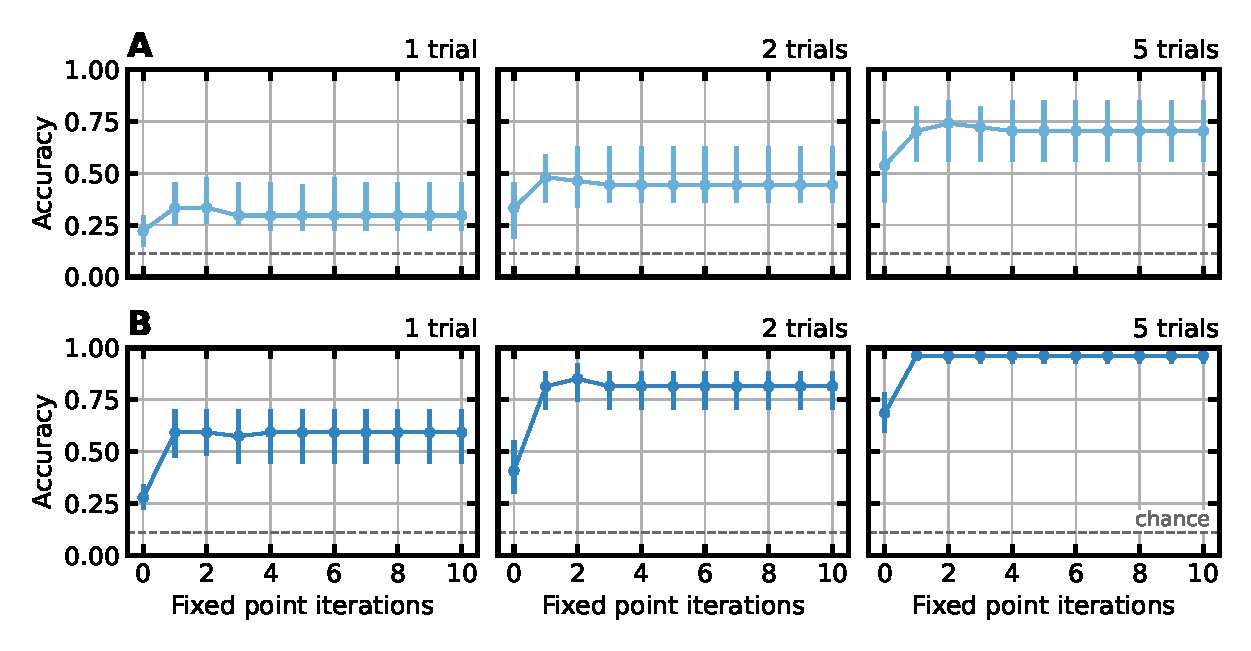
\includegraphics[width=\linewidth]{figures/fpi.eps}
		\caption{Average cross-validated \textsc{stbf-struct} Accuracy using
			one trial per block over all 21 subjects
			relative to the number of iterations used to estimate the Kronecker-Toeplitz structured shrunk
			covariance. Error bars represent the first and third quartiles. The
			accuracy does not improve when using more than one iteration.
			(\textbf{a}) Results for 1, 2, and 5 trials using only the first block in each
			training fold for training. (\textbf{b}) Results
			for 1, 2, and 5 trials using
			all nine training blocks in the training folds.
		}
		\label{fig:iterations}
	\end{figure}

	\subsection{Classifier accuracy for limited training data}
	It is of interest to keep the calibration time before BCI
	operation as short as possible.
	We mimic this problem by training the classifier with as few training epochs as possible.
	We evaluate the performance of all classifiers for different levels of
	available training data and apply the cross-validation procedure nine times (the number of blocks in the training fold) for all subjects, keeping the
	corresponding number of blocks in the training folds and dropping the rest.
	\autoref{fig:accuracy} and \autoref{ap:accuracy_ap} show each classifier's
	accuracy relative to the data availability.
	We statistically compare the two newly proposed classifiers,
	\textsc{stbf-struct} and \textsc{stbf-shrunk}, for different levels of training
	data availability using a one-sided paired Wilcoxon rank-sum test with Holm correction for the multiple pairwise comparisons between classifiers.
	We performed this analysis three times: by only using the first trial of a
	block, by averaging epochs across the first two trials of a block and across
	the first five trials of a block.
	Results validated on one trial are reported in \autoref{tab:p_values_1}, 2-trial results
	in \autoref{tab:p_values_2}, and 5-trial results in \autoref{tab:p_values_5}.

	\begin{figure}
		%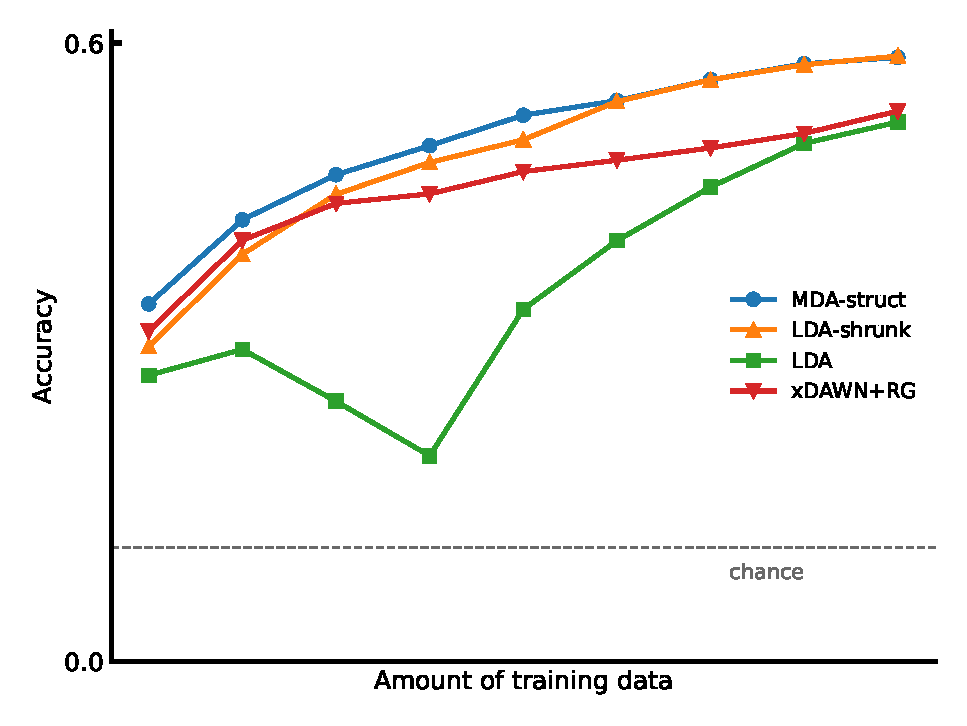
\includegraphics[width=\linewidth]{figures/accuracy.eps}
		\caption{Accuracy of the different classifiers for all 21 subjects relative to the
			number of blocks available for training. One block consists of 135
			epochs and corresponds to 27 seconds of stimulation. Accuracies
			are shown for the evaluation settings averaging over 1, 2, and
			3 trials of testing stimuli.
			\autoref{ap:accuracy_ap} contains results for all numbers of trials.
			While \textsc{stbf-emp} is unstable when little training data
			are available,
			regularization of the covariance matrix (\textsc{stbf-shrunk} and
			\textsc{stbf-struct}) drastically improves performance.}
		\label{fig:accuracy}
	\end{figure}
	\begin{table}[h]
		\centering
				\begin{tabularx}{\linewidth}{@{}lrrrrrrrrr@{}}
			\toprule
			1 Trial                                       & \multicolumn{9}{c}{Nb. of training blocks}                                                                                                         \\ \cline{2-10}
			                                              & 1                                          & 2          & 3          & 4          & 5          & 6          & 7          & 8          & 9          \\ \midrule
			\textsc{stbf-struct} $>$ \textsc{stbf-shrunk} & \pv{0.005}                                 & \pv{0.030} & \pv{0.015} & \pv{0.543} & \pv{0.284} & \pv{0.159} & \pv{1.000} & \pv{1.000} & \pv{0.952} \\
			\textsc{stbf-struct} $>$ \textsc{stbf-emp}    & \pv{0.000}                                 & \pv{0.000} & \pv{0.000} & \pv{0.000} & \pv{0.000} & \pv{0.000} & \pv{0.000} & \pv{0.000} & \pv{0.000} \\
			\textsc{stbf-struct} $>$ x\textsc{dawn-rg}    & \pv{0.086}                                 & \pv{0.002} & \pv{0.000} & \pv{0.000} & \pv{0.000} & \pv{0.000} & \pv{0.000} & \pv{0.000} & \pv{0.000} \\ \midrule
			\textsc{stbf-shrunk} $>$ \textsc{stbf-emp}    & \pv{0.000}                                 & \pv{0.000} & \pv{0.000} & \pv{0.000} & \pv{0.000} & \pv{0.000} & \pv{0.000} & \pv{0.000} & \pv{0.000} \\
			\textsc{stbf-shrunk} $>$ x\textsc{dawn-rg}    & \pv{1.000}                                 & \pv{0.499} & \pv{0.071} & \pv{0.000} & \pv{0.000} & \pv{0.000} & \pv{0.000} & \pv{0.001} & \pv{0.001} \\
			\bottomrule
		\end{tabularx}

		\caption{$p$-values calculated by one-sided paired Wilcoxon rank-sum test with
			Holm correction using one testing trial for different classifiers
			and levels of data availability. $p$-values $<0.05$ are considered significant
			and marked in grey.}
		\label{tab:p_values_1}

		\centering
				\begin{tabularx}{\linewidth}{@{}lrrrrrrrrr@{}}
			\toprule
			2 Trials                                      & \multicolumn{9}{c}{Nb. of training blocks}                                                                                                         \\ \cline{2-10}
			                                              & 1                                          & 2          & 3          & 4          & 5          & 6          & 7          & 8          & 9          \\ \midrule
			\textsc{stbf-struct} $>$ \textsc{stbf-shrunk} & \pv{0.014}                                 & \pv{0.006} & \pv{0.040} & \pv{0.040} & \pv{0.004} & \pv{0.846} & \pv{0.888} & \pv{1.000} & \pv{1.000} \\
			\textsc{stbf-struct} $>$ \textsc{stbf-emp}    & \pv{0.000}                                 & \pv{0.000} & \pv{0.000} & \pv{0.000} & \pv{0.000} & \pv{0.000} & \pv{0.000} & \pv{0.000} & \pv{0.000} \\
			\textsc{stbf-struct} $>$ x\textsc{dawn-rg}    & \pv{0.103}                                 & \pv{0.004} & \pv{0.000} & \pv{0.000} & \pv{0.000} & \pv{0.000} & \pv{0.000} & \pv{0.000} & \pv{0.000} \\ \midrule
			\textsc{stbf-shrunk} $>$ \textsc{stbf-emp}    & \pv{0.000}                                 & \pv{0.000} & \pv{0.000} & \pv{0.000} & \pv{0.000} & \pv{0.000} & \pv{0.000} & \pv{0.000} & \pv{0.000} \\
			\textsc{stbf-shrunk} $>$ x\textsc{dawn-rg}    & \pv{1.000}                                 & \pv{1.000} & \pv{0.163} & \pv{0.001} & \pv{0.001} & \pv{0.000} & \pv{0.000} & \pv{0.000} & \pv{0.000} \\
			\bottomrule
		\end{tabularx}

		\caption{$p$-values as in \autoref{tab:p_values_1} averaging over two testing trials.}
		\label{tab:p_values_2}

		\centering
				\begin{tabularx}{\linewidth}{@{}lrrrrrrrrr@{}}
			\toprule
			5 Trials                                      & \multicolumn{9}{c}{Nb. of training blocks}                                                                                                         \\ \cline{2-10}
			                                              & 1                                          & 2          & 3          & 4          & 5          & 6          & 7          & 8          & 9          \\ \midrule
			\textsc{stbf-struct} $>$ \textsc{stbf-shrunk} & \pv{0.005}                                 & \pv{0.030} & \pv{0.015} & \pv{0.543} & \pv{0.284} & \pv{0.159} & \pv{1.000} & \pv{1.000} & \pv{0.952} \\
			\textsc{stbf-struct} $>$ \textsc{stbf-emp}    & \pv{0.000}                                 & \pv{0.000} & \pv{0.000} & \pv{0.000} & \pv{0.000} & \pv{0.000} & \pv{0.000} & \pv{0.000} & \pv{0.000} \\
			\textsc{stbf-struct} $>$ x\textsc{dawn-rg}    & \pv{0.086}                                 & \pv{0.002} & \pv{0.000} & \pv{0.000} & \pv{0.000} & \pv{0.004} & \pv{0.006} & \pv{0.000} & \pv{0.000} \\ \midrule
			\textsc{stbf-shrunk} $>$ \textsc{stbf-emp}    & \pv{0.000}                                 & \pv{0.000} & \pv{0.000} & \pv{0.000} & \pv{0.000} & \pv{0.000} & \pv{0.000} & \pv{0.000} & \pv{0.000} \\
			\textsc{stbf-shrunk} $>$ x\textsc{dawn-rg}    & \pv{1.000}                                 & \pv{0.499} & \pv{0.000} & \pv{0.000} & \pv{0.000} & \pv{0.000} & \pv{0.000} & \pv{0.001} & \pv{0.001} \\
			\bottomrule
		\end{tabularx}

		\caption{$p$-values as in \autoref{tab:p_values_1} averaging over five testing trials.}
		\label{tab:p_values_5}
	\end{table}
	\unskip

	The tables show that \textsc{stbf-struct} has a significant advantage over
	\textsc{stbf-shrunk} when the number of training blocks is low.
	This effect is present for 1-, 2- and 5-trial evaluation.
	This advantage decreases (the $p$-value increases) when
	adding more training blocks.
	Both \textsc{stbf-struct} and \textsc{stbf-shrunk} perform significantly better
	than \textsc{stbf-emp} for all evaluated settings.
	Compared to x\textsc{dawn+rg}, \textsc{stbf-struct} also has significantly
	higher accuracy in almost all evaluated settings, except when using only one training block.
	\textsc{stbf-shrunk} does not outperform x\textsc{dawn+rg} when training data is low but gains a significant advantage
	when using more training data.

	\subsection{Classifier training time}
	In order to evaluate the training time of the investigated classifiers, the
	cross-validation scheme is run four times for each subject, each time with an
	increasing number of EEG channels retained in the analysis, to explore the scalability of each classifier for analyses with higher spatial resolutions.
	The temporal resolutions were not varied, but we expect that increasing the
	temporal resolution has a similar effect on training time since the
	training times for the \textsc{stbf}-based as evidenced by the complexity
	calculations in \autoref{sec:parameters_complexity}.
	\autoref{fig:training_time} shows the measured training times.
	These results were obtained using a laptop with an Intel® Core™ i7-8750H CPU and 16GB of RAM.

	\begin{figure}
		%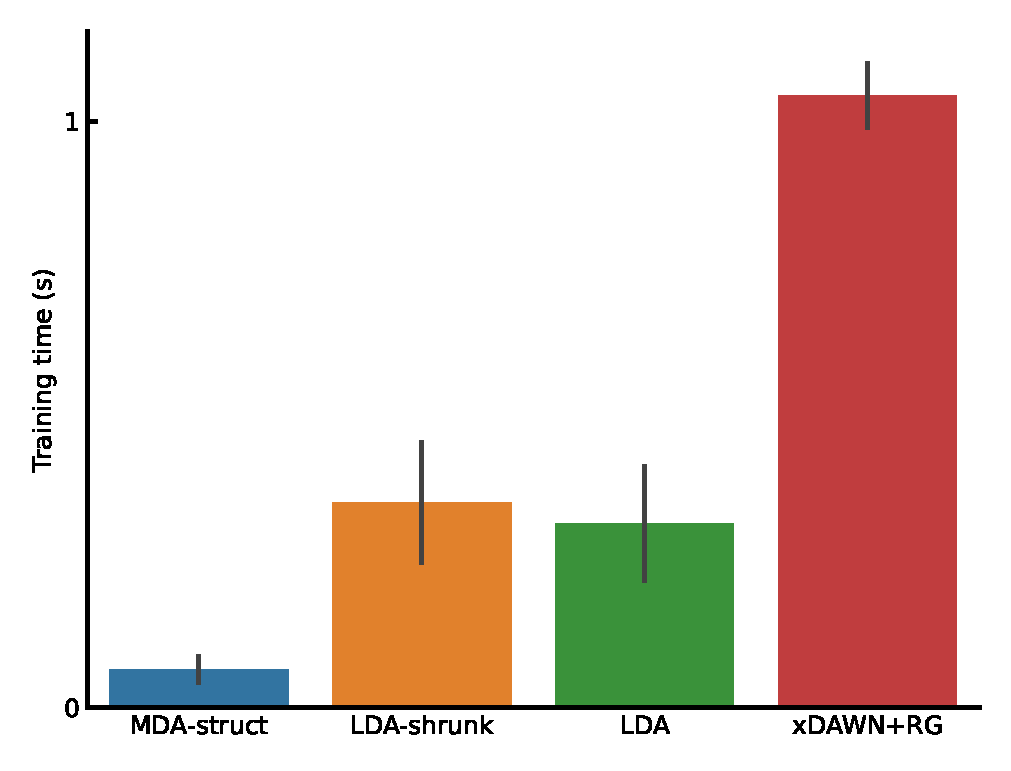
\includegraphics[width=\linewidth]{figures/training_time.eps}
		\caption{Median fold training time for different classifiers at different spatial
			resolution levels evaluated over all training folds for all subjects.
			Error bars represent standard deviation. The training time of \textsc{stbf-shrunk} increases more
			steeply with resolution compared to \textsc{stbf-struct}.
			All \textsc{stbf} classifiers can be trained significantly faster than
			x\textsc{dawn+rg}.}
		\label{fig:training_time}
	\end{figure}

	\autoref{fig:training_time} shows that the training time of
	\textsc{stbf-struct} increases less steeply than that of \textsc{stbf-shrunk}
	and \textsc{stbf-emp}. The training time of all three STBF-based classifiers is
	much lower than that of x\textsc{dawn+rg}, which appears nearly constant when using
	4, 8, 16, or 32 channels.

	\section{Discussion}

	\subsection{Classification accuracy}
	As evidenced by \autoref{fig:accuracy} and Tables \ref{tab:p_values_1}-\ref{tab:p_values_5}, the regularized classifiers \textsc{stbf-shrunk}
	and \textsc{stbf-struct} significantly improve the classification accuracy
	compared to the original \textsc{stbf-emp} for all numbers of training blocks
	indicated.
	We believe there are three reasons for this.
	First and foremost, the empirical covariance matrix in \textsc{stbf-emp} becomes
	ill-conditioned when the number of available training epochs is smaller than
	the number of features ($n<cs$), rendering its inversion with the
	Moore-Penrose pseudoinverse unstable.
	This is the case \textsc{stbf-emp} when $n=cs=32*17=544$, after which the
	accuracy of \textsc{stbf-emp} starts to increase.
	This effect is visible in \autoref{fig:accuracy}, where the accuracy starts
	increasing when using more than four training blocks, amounting to 540 epochs.
	The noticeable dip in accuracy when using around 540 epochs can be explained by
	numerical effects in the pseudoinverse for very small
	eigenvalues~\cite{Blankertz2011, Raudys1998, Schaefer2004,
		Kraemer2009}.
	Regularization of the covariance matrix with shrinkage ensures that the
	covariance matrix is non-singular and better conditioned so it can stably be inverted.
	Second, covariance regularization introduces a trade-off between variance and bias of the model~\cite{Ledoit2004}.
	Better performance on unseen data can be achieved when some model variance is
	traded for extra bias.
	Regularization reduces extreme values present, as shown in
	\autoref{fig:kronlda-covs}, resulting in a classifier with
	better generalization.
	Third, the true spatiotemporal covariance matrix may vary throughout BCI
	sessions, e.g., due to movement of the EEG-cap, changing impedances of
	electrodes, subject fatigue, the introduction of new spatiotemporal noise
	sources, and other possible confounds.
	A regularized covariance matrix should better account for changes in true covariance.
	Note that the LOOCV method in principle assumes that the covariances of
	the training data and unseen data are the same.
	Because the covariance might have changed for unseen data, the shrinkage
	estimate obtained with LOOCV is probably still an
	underestimation of the optimal -- but unknown -- shrinkage coefficient that
	would yield the best classification accuracy for the unseen data.

	Another observation is the significantly better accuracy score of
	\textsc{stbf-struct} over \textsc{stbf-shrunk} when the amount of available training data is small.
	This property is an attractive advantage in a BCI setting since it is desirable to keep the calibration (training) phase as short as possible without losing accuracy.
	The accuracy advantage of the structured estimator is a consequence of the
	Kronecker-Toeplitz covariance structure, which is informative for the
	underlying process generating the epochs, if it is assumed that the EEG signal
	is a linear combination of stationary activity generated by random dipoles in
	the brain with added noise~\cite{Munck1992, DeMunck2002, GonzalezNavarro2017}.
	Hence, \textsc{stbf-struct} can utilize this prior information to better estimate the inverse
	covariance.
	The increase in accuracy for small training set sizes can also be explained by the smaller number of parameters necessary to estimate the inverse covariance (see \autoref{sec:parameters_complexity}), increasing the stability of matrix inversions.

	When compared to the state-of-the-art x\textsc{dawn+rg} classifier, we conclude
	that \textsc{stbf-struct} reaches similar accuracy when using only one block of
	training data.
	The authors suspect this is due to both
	classifiers having insufficient training information to reach
	satisfactory classification accuracy.
	When more data are available, \textsc{stbf-struct} reaches significantly better accuracies.
	Combined with the benefits laid out in  \autoref{sec:parameters_complexity} and
	\autoref{sec:interpretability}, this makes it an attractive option for ERP classification.
	\textsc{stbf-shrunk} does not show decisive accuracy improvements over
	x\textsc{dawn+rg} using a few training blocks, but this improves as the training data increases.

	\subsection{Time and memory complexity}
	\label{sec:parameters_complexity}
	As mentioned above, inverting the full $cs \times cs$ dimensional covariance
	matrix to construct \textsc{stbf-emp} and \textsc{stbf-shrunk} can be costly
	and unstable, in particular in high-resolution settings with many EEG channels or time samples.
	Constructing the full covariance and inverse covariance matrices also requires a considerable amount of memory.
	The structured covariance estimator of \textsc{stbf-struct} has two advantages here.

	First, because of \autoref{prop:inverse_kronecker} and
	\autoref{prop:kronecker_multiplication} there is no need to calculate or keep in memory the full $cs\times cs$
	symmetric covariance and inverse covariance matrices for \textsc{stbf-struct}; they can instead be replaced by two smaller symmetric matrices respectively of dimensions $c\times c$ and $s\times s$.
	Furthermore, since the temporal component of the Kronecker product is
	Toeplitz-structured, it only requires $s$ parameters to
	estimate.
	While the inverse covariance of \textsc{stbf-emp} and \textsc{stbf-shrunk} is
	defined by $\frac{cs(cs+1)}{2}=\frac{32\cdot17(32\cdot17+1)}{2}=\num{122128}$
	parameters accounting for the symmetric nature of
	covariance, the structured estimator only requires $\frac{c(c+1)}{2} + s =
		\frac{32(32+1)}{2} + 17=545$ unique parameters.
	This reduction in parameters to estimate reduces memory usage and contributes to the regularization effect for low data availability settings.
	The inverse covariances of \textsc{stbf-emp} and
	\textsc{stbf-struct}, represented as $32*17\times 32*17$ symmetric matrices of
	single-precision real floating point numbers for weight calculation,
	use 9.03MiB of memory.
	The $32\times 32$ and $17\times 17$ matrices of \textsc{stbf-struct} only
	require 5.12KiB.

	Second, structured estimation has better time complexity.
	Covariance estimation and inversion occupy the largest part of the STBF training time.
	For \textsc{stbf-emp} and \textsc{stbf-shrunk}, the time complexity of this process is $\mathcal{O}(nc^2s^2+c^3s^3)$.
	Thanks to Property~\ref{prop:inverse_kronecker}, the complexity can be reduced to
	$\mathcal{O}(nc^2s^2+c^3+s^3)$ for the structured estimator of \textsc{stbf-struct}.
	The results presented in \autoref{fig:training_time} confirm these
	calculations.
	It can be observed that the training time of \textsc{stbf-struct} stays low compared to \textsc{stbf-emp} and \textsc{stbf-shrunk} when dimensionality increases.

	The results shown in \autoref{fig:training_time} also confirm that the
	STBF-based estimators are very fast to train compared to the
	state-of-the-art estimator x\textsc{dawn+rg}, which confirms the results in~\cite{Wittevrongel2016}.
	Since the training times of all STBF-based classifiers are already in
	the order of tenths of seconds, the question arises whether the
	improvements achieved by using the structured estimator would be relevant in
	practice.
	However, the authors believe that these results could significantly impact some
	use cases of the spatiotemporal beamformer, like high spatial or temporal resolution ERP analyses.
	One example is single-trial ERP analysis with a high-temporal
	resolution to extract ERP time features.
	Such higher-resolution analyses can later be incorporated into an ERP
	classification framework.
	In addition, the speed-up provided by structured estimation yields a faster
	off-line evaluation of the STBF ERP classifier, where often multiple cross-validation folds, subjects, and hyperparameter settings need to be explored, which can quickly increase runtime.
	Improvements in computation speed and memory usage can remove the need for dedicated computation hardware and enable running group analyses on a personal computer.

	%	\subsection{Interpreting the weights}
	%	\label{sec:interpretability}
	%	The weight matrix of the STBF determines how each
	%	spatiotemporal feature of a given epoch should contribute to enhancing the SNR
	%	of the discriminating signal in the classification
	%	task.
	%	Alternatively, the activation pattern can be regarded as a forward EEG model of
	%	the activity generating the discriminating signal and the weights as a
	%	backward model~\cite{Blankertz2011,Haufe2014}.
	%	Regularization enables a researcher to interpret better the distribution of the weight over space and time after reshaping the weight vector $\mathbf{w}$ to its spatiotemporal matrix equivalent $W$ such that $\text{vec}(W) = \mathbf{w}$.
	%	\autoref{fig:interpret_weights} compares the weights calculated in
	%	\textsc{stbf-emp} and \textsc{stbf-shrunk} with the weights from
	%	\textsc{stbf-struct}.
	%
	%	\begin{figure}
	%		%\includegraphics[width=\linewidth]{figures/weights.eps}
	%		\caption{Spatiotemporal beamformer weights calculated using four
	%			blocks of data (of 1215 epochs) from \textit{Subject 01} from
	%			0.2s before to 1.0s after stimulus onset.
	%			Regularized weights show an interpretable sparse pattern,
	%			while the empirical weights appear noisier.
	%			(\textbf{a}) Spatiotemporal activation pattern with spatial and temporal global field
	%			power.
	%			(\textbf{b}) \textsc{stbf-struct} weights with spatial and temporal average of
	%			absolute values.
	%			(\textbf{c}) \textsc{stbf-shrunk} weights. The shrinkage factor $\alpha=0.05$ was
	%			determined with the closed-form LOOCV-method.
	%			(\textbf{d}) \textsc{stbf-emp} weights.}
	%		\label{fig:interpret_weights}
	%	\end{figure}
	%
	%	Since the linear filter's noise suppression and signal amplification functions are deeply entangled, it is not necessarily true that features with a
	%	high filter weight directly correlate to features containing discriminatory
	%	information~\cite{Haufe2014}.
	%	However, it still is possible to interpret the weights in terms of which
	%	features contribute most to the classification process, be it through noise
	%	suppression, signal amplification, or -- most likely -- a combination of both.
	%	The weights obtained by \textsc{stbf-emp} look randomly distributed over space
	%	and time; the regularized estimator used by \textsc{stbf-shrunk} and
	%	\textsc{stbf-struct} reveal a more interpretable weight distribution.
	%	The \textsc{stbf-shrunk} weights show a sparse spatial distribution while
	%	the \textsc{stbf-struct} weights show a sparse distribution in both space and in
	%	time.
	%
	%	As expected, \autoref{fig:interpret_weights}b and d exhibit weight around
	%	the central and parietal regions, where the P300 ERP component is present.
	%	Especially the spatial weights of \textsc{stbf-shrunk} in
	%	\autoref{fig:interpret_weights}d correspond to the spatial activation pattern
	%	in \autoref{fig:interpret_weights}a.
	%	This is not unsurprising, since shrinkage transforms the covariance matrix closer to the
	%	identity matrix and assuming identity covariance in \autoref{eq:closed_form} yields weights
	%	identical to the activation pattern (up to a scaling factor).
	%	Additionaly, \autoref{fig:interpret_weights}b shows that weights in the baseline interval and after 0.6s, which should
	%	contain no response information, are close to zero for the structured estimator.
	%	Meanwhile, these weights are high in the occipital region between 0.1s and 0.2s,
	%	containing early visual components with relatively low SNR.
	%	This high weight for the early visual components confirms the results from Treder \& Blankertz~\cite{Treder2010}
	%	that state that, in addition to the P300, the early N1 and P2 ERP components
	%	are also modulated by oddball attention and contain discriminatory information between
	%	attended and non-attended stimuli.
	%
	%	Using an interpretable classification model has many advantages.
	%	For instance, one can use the weight matrix determine relevant time samples
	%	and EEG channels for per-subject feature selection to refine the model further .
	%	The number of channels is also an important cost factor in practical BCI
	%	applications.
	%	Determining which channels do not contribute to the classification accuracy
	%	helps reduce the number of required electrodes.
	%	Spatially clustered weights indicate that some electrodes are not used by the
	%	classifier and can be discarded accordingly with no substantial accuracy
	%	reduction.
	%	As another example, information about the timing and spatial distribution of
	%	the discriminatory information in the response can be extracted from the
	%	weights
	%	and linked neurophysiological hypotheses.

	\todo{Remove mentions of interpretability}

	\section{Conclusion}
	While it is possible to regularize the spatiotemporal LCMV beamformer
	classifier for ERP detection with other methods such as by employing feature selection,
	by adding regularizing penalties to the cost
	function beamforming problem, or by crafting a cleaner activation pattern, our work focused on
	estimation methods for the spatiotemporal covariance.
	We introduced a covariance estimator using adaptive shrinkage and an
	estimator exploiting prior knowledge about the spatiotemporal nature of the EEG
	signal.
	We compared these estimators with the original spatiotemporal
	beamformer and a state-of-the-art method in an off-line P300 detection task.
	Our results show that the structured estimator performs better when training data are sparsely available and that it can be computed faster and with substantially less memory usage.
	Since these algorithms are not paradigm-specific,  the conclusions can be generalized to
	other ERP-based BCI settings.

	Future work should focus on introducing more robust regularization strategies using prior knowledge, such as shrinking the spatial covariance to a population mean or a priorly known matrix based on sensor geometry or characterizing the temporal covariance as a wavelet or autoregressive model.
	More accurate results could be obtained by expressing the covariance as the sum of multiple Kronecker products to account for spatial variation in temporal
	covariance.
	It could also be interesting to explore the impact of covariance regularization on transfer learning of the STBF between subjects to alleviate calibration entirely.
	Finally, it could be insightful to evaluate the proposed algorithms in a
	real-world on-line BCI setting.

	\todo{check chapters/structure paper}
	\todo{check structure Leuven.ai poster}
	\section{The spatiotemporal EEG covariance}
	\section{The single-KP covariance model}
	\section{The sum-of-KP covariance model}
	\section{Decoding performance}
	\subsection{Extension into the space-time-frequency domain}
	\printbibliography
\end{refsection}
